\documentclass[12pt,letterpaper]{article}
\usepackage{graphicx,textcomp}
\usepackage{natbib}
\usepackage{setspace}
\usepackage{fullpage}
\usepackage{color}
\usepackage[reqno]{amsmath}
\usepackage{amsthm}
\usepackage{fancyvrb}
\usepackage{amssymb,enumerate}
\usepackage[all]{xy}
\usepackage{endnotes}
\usepackage{lscape}
\newtheorem{com}{Comment}
\usepackage{float}
\usepackage{hyperref}
\newtheorem{lem} {Lemma}
\newtheorem{prop}{Proposition}
\newtheorem{thm}{Theorem}
\newtheorem{defn}{Definition}
\newtheorem{cor}{Corollary}
\newtheorem{obs}{Observation}
\usepackage[compact]{titlesec}
\usepackage{dcolumn}
\usepackage{tikz}
\usetikzlibrary{arrows}
\usepackage{multirow}
\usepackage{xcolor}
\newcolumntype{.}{D{.}{.}{-1}}
\newcolumntype{d}[1]{D{.}{.}{#1}}
\definecolor{light-gray}{gray}{0.65}
\usepackage{url}
\usepackage{listings}
\usepackage{color}

\definecolor{codegreen}{rgb}{0,0.6,0}
\definecolor{codegray}{rgb}{0.5,0.5,0.5}
\definecolor{codepurple}{rgb}{0.58,0,0.82}
\definecolor{backcolour}{rgb}{0.95,0.95,0.92}

\lstdefinestyle{mystyle}{
	backgroundcolor=\color{backcolour},   
	commentstyle=\color{codegreen},
	keywordstyle=\color{magenta},
	numberstyle=\tiny\color{codegray},
	stringstyle=\color{codepurple},
	basicstyle=\footnotesize,
	breakatwhitespace=false,         
	breaklines=true,                 
	captionpos=b,                    
	keepspaces=true,                 
	numbers=left,                    
	numbersep=5pt,                  
	showspaces=false,                
	showstringspaces=false,
	showtabs=false,                  
	tabsize=2
}
\lstset{style=mystyle}
\newcommand{\Sref}[1]{Section~\ref{#1}}
\newtheorem{hyp}{Hypothesis}

\title{Problem Set 2}
\date{Due: October 3, 2022}
\author{Daniel Murray (13303981)}

\begin{document}
	\maketitle
	\section*{Instructions}
\begin{itemize}
	\item Please show your work! You may lose points by simply writing in the answer. If the problem requires you to execute commands in \texttt{R}, please include the code you used to get your answers. Please also include the \texttt{.R} file that contains your code. If you are not sure if work needs to be shown for a particular problem, please ask.
	\item Your homework should be submitted electronically on GitHub.
	\item This problem set is due before 23:59 on Sunday October 16, 2022. No late assignments will be accepted.
	\item Total available points for this homework is 80.
\end{itemize}

	
	\vspace{.5cm}
	\section*{Question 1 (40 points): Political Science}
		\vspace{.25cm}
	The following table was created using the data from a study run in a major Latin American city.\footnote{Fried, Lagunes, and Venkataramani (2010). ``Corruption and Inequality at the Crossroad: A Multimethod Study of Bribery and Discrimination in Latin America. \textit{Latin American Research Review}. 45 (1): 76-97.} As part of the experimental treatment in the study, one employee of the research team was chosen to make illegal left turns across traffic to draw the attention of the police officers on shift. Two employee drivers were upper class, two were lower class drivers, and the identity of the driver was randomly assigned per encounter. The researchers were interested in whether officers were more or less likely to solicit a bribe from drivers depending on their class (officers use phrases like, ``We can solve this the easy way'' to draw a bribe). The table below shows the resulting data.

\newpage
\begin{table}[h!]
	\centering
	\begin{tabular}{l | c c c }
		& Not Stopped & Bribe requested & Stopped/given warning \\
		\\[-1.8ex] 
		\hline \\[-1.8ex]
		Upper class & 14 & 6 & 7 \\
		Lower class & 7 & 7 & 1 \\
		\hline
	\end{tabular}
\end{table}

\begin{enumerate}
	
	\item [(a)]
	Calculate the $\chi^2$ test statistic by hand/manually (even better if you can do "by hand" in \texttt{R}).\\
	
	\textbf{Answer:}
	
	The $\chi^2$ test statistic was calculated manually in \texttt{R}, using the code below. The value for the $\chi^2$ test statistic was found to be 3.79.
	
	\vspace{.5cm}
	
	\lstinputlisting[language=R, firstline=7, lastline=47]{PS02.R}  
	
	\vspace{.5cm}
	
	\item [(b)]
	Now calculate the p-value from the test statistic you just created (in \texttt{R}).\footnote{Remember frequency should be $>$ 5 for all cells, but let's calculate the p-value here anyway.}  What do you conclude if $\alpha = 0.1$?\\
	
	\textbf{Answer:}
	
	The degrees of freedom was first calculated by multiplying the number of rows minus one by the number of columns minus one, and was found to equal 2. The P-value was then calculated using the \texttt{pchisq} function. Its value was found to be approximately 0.15.
	
	The code below illustrates this process:
	
	\vspace{.5cm}
	
	\lstinputlisting[language=R, firstline=51, lastline=57]{PS02.R}  
	
	\vspace{.5cm}
	
	As the p-value ($\approx 0.15$) is higher than our $\alpha = 0.1$ threshold, we do not find sufficient evidence to reject the null hypothesis that there is no relationship between a driver's class and the likelihood of an officer soliciting a bribe after committing a minor traffic offence.
	
	\newpage
	\item [(c)] Calculate the standardized residuals for each cell and put them in the table below.
	\vspace{0.5cm}
	
	\textbf{Answer:}\\
	
	\begin{table}[h]
		\centering
		\begin{tabular}{l | c c c }
			& Not Stopped & Bribe requested & Stopped/given warning \\
			\\[-1.8ex] 
			\hline \\[-1.8ex]
			Upper class  & 0.32 & -1.64 & 1.52 \\
			\\
			Lower class & -0.32 & 1.64  & -1.52  \\
			
		\end{tabular}
	\end{table}

	\vspace{.5cm}

	The code below was used to calculate the standardised residuals in \texttt{R}:
	
	\vspace{.5cm}
		
	\lstinputlisting[language=R, firstline=63, lastline=75]{PS02.R}  
	
	\vspace{.5cm}
		
	\item [(d)] How might the standardized residuals help you interpret the results?\\  
	
	\textbf{Answer:}\\
	
	Whereas the $\chi^2$ test statistic summarises how close the observed frequencies are to the expected frequencies over all cells in the contingency table, the standardised residuals help us to understand the pattern of association among the individual cells. When $H_0$ (independence) is true, the standardised residuals would have a normal standard distribution. This means that there is a very small probability (approximately 5\%) of their values being larger than 2 in absolute value.
	
	In the case of our data, the standardised residuals are all less than 2 in absolute value. This suggests that no individual cell has too many or too few observations to indicate a departure from independence between the variables.
	
\end{enumerate}
\newpage

\section*{Question 2 (40 points): Economics}
Chattopadhyay and Duflo were interested in whether women promote different policies than men.\footnote{Chattopadhyay and Duflo. (2004). ``Women as Policy Makers: Evidence from a Randomized Policy Experiment in India. \textit{Econometrica}. 72 (5), 1409-1443.} Answering this question with observational data is pretty difficult due to potential confounding problems (e.g. the districts that choose female politicians are likely to systematically differ in other aspects too). Hence, they exploit a randomized policy experiment in India, where since the mid-1990s, $\frac{1}{3}$ of village council heads have been randomly reserved for women. A subset of the data from West Bengal can be found at the following link: \url{https://raw.githubusercontent.com/kosukeimai/qss/master/PREDICTION/women.csv}\\

\noindent Each observation in the data set represents a village and there are two villages associated with one GP (i.e. a level of government is called "GP"). Figure~\ref{fig:women_desc} below shows the names and descriptions of the variables in the dataset. The authors hypothesize that female politicians are more likely to support policies female voters want. Researchers found that more women complain about the quality of drinking water than men. You need to estimate the effect of the reservation policy on the number of new or repaired drinking water facilities in the villages.
\vspace{.5cm}
\begin{figure}[h!]
	\caption{\footnotesize{Names and description of variables from Chattopadhyay and Duflo (2004).}}
	\vspace{.5cm}
	\centering
	\label{fig:women_desc}
	
\end{figure}		

\newpage
\begin{enumerate}
	\item [(a)] State a null and alternative (two-tailed) hypothesis.\\
	
	\textbf{Answer:}\\
	
	As we are using a bivariate linear regression, we want our null hypothesis to reflect "no effect" for our $\beta$ coefficient estimate. In other words, it states that our $\beta$ coefficient estimate is equal to zero; there is no statistically significant relationship between x and y. As we want our alternative hypothesis to be two-tailed, it will simply state that our $\beta$ coefficient estimate is not equal to zero, rather than indicating any particular directionality. It states that there is a statistically significant relationship between x and y.\\
	
	Below are our null and alternative (two-tailed) hypotheses:
	
	\[H_0: \beta = 0 \]
	\[H_a : \beta \neq 0 \]
	
	\vspace{.5cm}

	\item [(b)] Run a bivariate regression to test this hypothesis in \texttt{R} (include your code!).\\
	
	\textbf{Answer:}\\
	
	We begin by creating a separate data frame to include only data for GPs reserved for female leaders and GPs with a male leader. This is to remove GPs not reserved for female leaders but which have a female leader, as these GPs are thought to have potential confounding problems. We do this by subsetting the dataset and combining the two subsets using the \texttt{rbind} function
	
	Next we use the \texttt{lm} function to run a bivariate linear regression with "water" as the response variable (y) and "female" as the explanatory variable (x).
	
	\vspace{.5cm}
	
	\lstinputlisting[language=R, firstline=89, lastline=97]{PS02.R}
	
	\vspace{.5cm}
	
	 \texttt{summary(ols)} in the code above produces the below output:\\
	 
	 \vspace{.5cm}
	 
	 \begin{figure}[H]\centering
	 	\caption{\footnotesize Summary of lm() function output}
	 	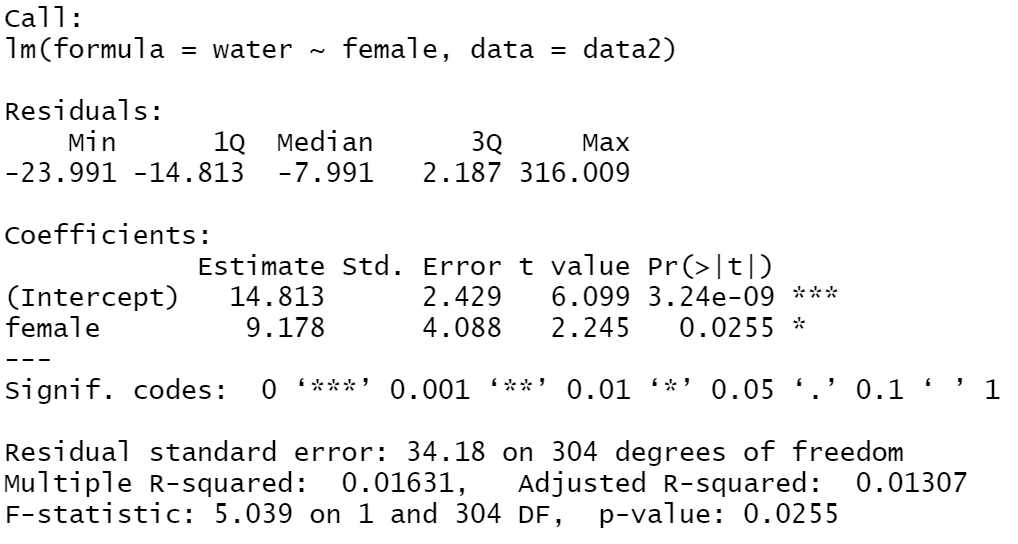
\includegraphics[width=.75\textwidth]{lm_output.png}
	 \end{figure} 
 
 	\vspace{.5cm}
 
  	We can also calculate our $\alpha$ and $\beta$ coefficients by hand in \texttt{R} using the code below: 
	
	\vspace{.5cm}
	
	\lstinputlisting[language=R, firstline=99, lastline=104]{PS02.R}
	
	\vspace{.5cm}
	
	This gives the same values as Figure 2 above, with $\alpha$ = 14.813 and $\beta$ = 9.178.\\
	
	\item [(c)] Interpret the coefficient estimate for reservation policy.\\ 
	
	\textbf{Answer:}\\
	
	In order to draw conclusions about our coefficient estimate for reservation police ($\beta$ = 9.178), we construct a 95\% confidence interval for its values. This has the following formula:
	
	\[\beta \pm t(se) \]
	
	Using a T table, we find the t-value for two-tailed 0.05 significance level at 304 degrees of freedom (n-2). This value is 1.9678.
	
	Next we calculate the standard error of beta by dividing the residual standard error of the regression by the square root of the total sum of squares for x. The code below shows these calculations:
	
	\vspace{.5cm}
	
	\lstinputlisting[language=R, firstline=108, lastline=118]{PS02.R}
	
	\vspace{.5cm}
	
	This give us a value of 4.088 for the standard error for $\beta$. Using these values we can now calculate our confidence interval, as below:
	
	\[\beta \pm t(se) \]
	\[9.178 \pm 1.9678 * 4.088 \]
	\[9.178 \pm 8.044 \]
	
	Our 95\% confidence interval for $\beta$ is (1.13, 17.22). As this confidence interval does not contain 0, we reject the null hypothesis and conclude that at the 95\% confidence level, there is a statistically significant positive association between reservation policy and the number of new or repaired drinking water facilities in villages. At a 95\% confidence level, we find that villages with female leadership have on average between 1.1 and 17.2 more new or repaired drinking water facilities than villages with male leadership, with our best estimate being an additional 9.2 water facilities.
	
\end{enumerate}

\end{document}
